% =========================================================================== %
\chapter{Описание реализованных средств}\label{chap4_soft_testing}
% =========================================================================== %
% --------------------------------------------------------------------------- %
\section{Описание реализованных алгоритмов}\label{sec:algorithm_desc}
% --------------------------------------------------------------------------- %

Сначала был разработан упрощённый алгоритм обхода, поддерживающий только условное ветвление. Его блок-схема представлена на рисунке~\ref{fig:flowchartNoBranching}.
\begin{figure}[!ht]
    \centering
    \includegraphics[height=0.6\textheight]{figures/flowchart.graphRunning1.png}
    \caption{Блок-схема алгоритма обхода графовой модели, не предполагающей параллельное исполнение}
    \label{fig:flowchartNoBranching}
\end{figure}

Далее был отдельно рассмотрен случай, когда необходимо параллельно обойти несколько ветвей. Для контроля за параллельным исполнением функций перехода и выполнения необходимых операций по распределению и сбору данных с задействованных вычислительных ресурсов была разработана управляющая струкутура <<контейнер выполнения>>. Более подробно структура описана в разделе~\ref{chap3_soft_architecture}. Логика работы с данной структурой представлена на рисунке~\ref{fig:flowchartExecutionContainer}.
\begin{figure}[H]
    \centering
    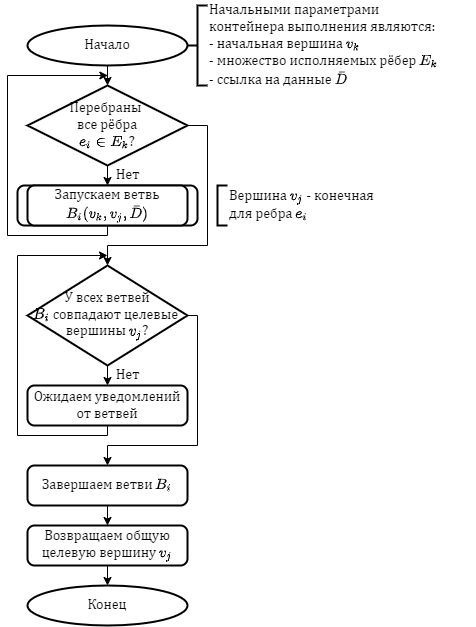
\includegraphics[height=0.6\textheight]{figures/flowchart.executionContainer.png}
    \caption{Блок-схема алгоритма отслеживания параллельного исполнения ветвей графа}
    \label{fig:flowchartExecutionContainer}
\end{figure}

При этом внутри управляющей структуры <<контейнер выполнения>> подразумевается создание отдельных <<ветвей>>.

Алгоритм обхода одной ветви представлен на рисунке~\ref{fig:flowchartExecutionBranch}.

\begin{figure}[H]
    \centering
    \includegraphics[width=0.8\textwidth]{figures/flowchart.executionBranch.png}
    \caption{Блок-схема алгоритма исполнения одной из параллельных ветвей}
    \label{fig:flowchartExecutionBranch}
\end{figure}

Общий алгоритм предполагает завершение выполнения ветви по сигналу от <<контейнера выполнения>>. Ситуация, когда по какой-то причине для текущей вершины $v_i$ и данных $\bar{D}$ не было выбрано ни одного ребра, является исключительной и должна обрабатываться отдельно.

% --------------------------------------------------------------------------- %
\section{Сборка и тестирование}
% --------------------------------------------------------------------------- %
Для сборки разработанных программных средств требуется библиотека Boost, компилятор языка С++, поддерживающий стандарт C++-11, и система сборки CMake. При разработке и отладке использовался компилятор gcc и библиотека Boost версии 1.78.

Для реализованных компонентов были разработаны unit-тесты для проверки корректности их внутренней логики. Разработанные юнит-тесты были размещены в директории comsdk/test (см. рисунок~\ref{fig:fileStructure}). Для выполнения тестирования использовалась система CTest.